\chapter{塑闪阵列探测器分系统的设计}
\label{ch:description}
塑闪阵列探测器(Plastic Scintillator Detector, 以下将简称PSD)是暗物质粒子探测卫星的关键子探测器之一,它位于DAMPE卫星的最顶部。
PSD需要实现以下两个功能:一是作为电荷测量探测器,对$Z=1\sim20$的入射相对论重离子进行鉴别;二是作为反符合探测器,区分电子和光子事件。
由于不同种类的入射粒子在物质中的沉积能量并不一致,PSD通过准确测量沉积能量的大小可以实现上述两个功能。

塑闪阵列探测器分系统可以分为4个功能模块,分别是塑闪阵列探测器主体功能模块、高压扇出板功能模块、前端电子学功能模块和机械支撑功能模块。
这些功能模块不仅实现了PSD的探测功能,而且为其正常运行提供了支撑环境。

本章将详细阐述PSD的工作原理及其结构组成,并给出DAMPE对PSD的性能要求。

\section{PSD的工作原理}
\label{sec:description:psd_principle}
PSD使用\SI{10}{\milli\meter}厚的有机塑料闪烁体作为探测器介质材料。
有机塑料闪烁体由于具有强的抗辐照特性、快的时间响应性、好的均匀性、长的光衰减长度、光输出高且易于加工等属性,在空间探测系统中常被用于提供系统的触发信号、能量测量及飞行时间测量。
入射粒子穿过塑料闪烁体时,与其中的原子(或离子,分子)发生相互作用而损失能量,并使得闪烁体中的原子(或离子,分子)激发到高能级。
受激的原子(或离子,分子)并不稳定,之后在从高能级跃迁到低能级的过程中以光子的形式释放能量(一般在可见光波段)。
这样,入射粒子在塑料闪烁体中的沉积能量就被转化成了光脉冲信号,并且沉积能量越大,产生的光子数越多。

光信号需要转换成电信号才能被电子学线路处理和采集。
PSD使用光电倍增管(photomultiplier tube,以下简称PMT)作为有机塑料闪烁体的读出器件。
PMT是粒子物理实验中一种常用的光电转换器件,它具有结构简单、增益高、线性范围广以及对单光子敏感等优点,并且在空间实验中有广泛的使用经验。
塑料闪烁体产生的闪烁光子被PMT接收后,经过光电转换、电子收集和倍增一系列过程,最终被转换成可以处理的电流脉冲信号输出。

PSD的前端电子学模块对来自PMT的电流信号进行电荷积分,然后放大、成形,最终将其幅度大小采集并保存下来。
由于PMT电流信号携带的电荷量与入射的闪烁光子数成正比,而闪烁光子数又与沉积能量的大小直接关联,这样PSD就实现了对入射粒子沉积能量的测量。

下面对PSD通过沉积能量大小进行粒子鉴别的物理原理以及PMT的工作原理进行介绍,这些是理解PSD设计的关键。

\subsection{重离子鉴别的原理}
\begin{figure}[h!]
	\centering
	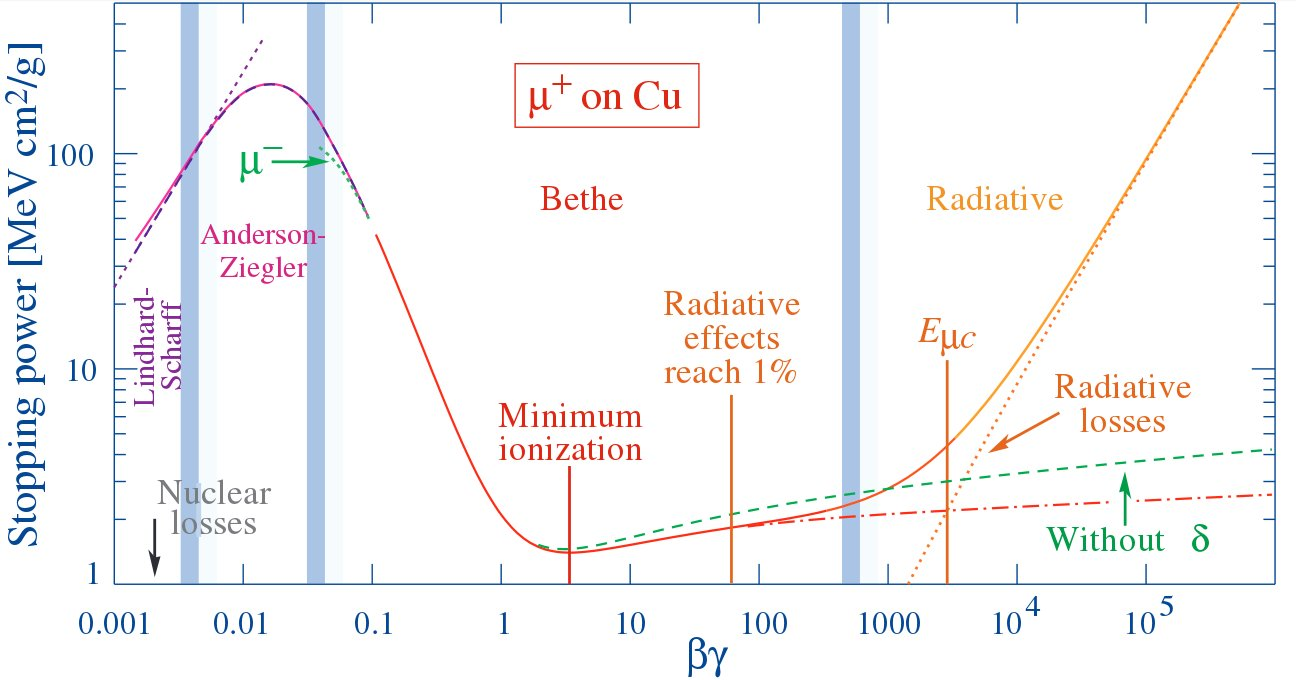
\includegraphics[width=0.8\linewidth]{chap/description/fig/energyloss_vs_velocity}
	\caption{${\mu}^+$在Cu中的能量损失率与速度的关系(用$\beta\gamma$表示),引自\parencite{pdg_book}。 图中实线是总的能量损失率,包含了所有相互作用。}
	\label{fig:description:energyloss_vs_velocity}
\end{figure}

\begin{figure}[h!]
	\centering
	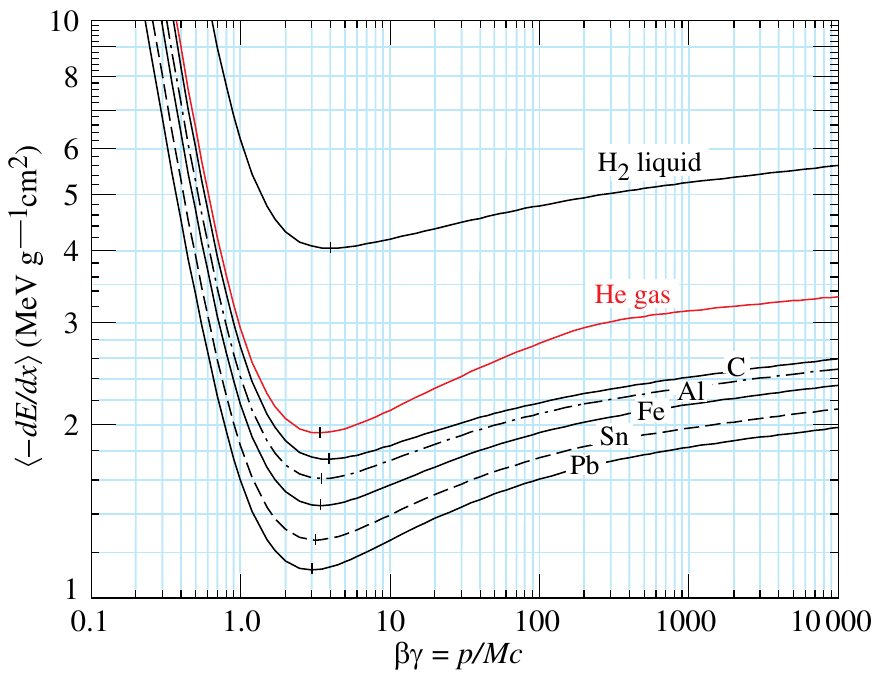
\includegraphics[width=0.8\linewidth]{chap/description/fig/fermi_plateau}
	\caption{入射粒子在几种不同介质中的电离能量损失随入射粒子动量的变化,可以清楚地看到费米坪,引自\parencite{pdg_book}。}
	\label{fig:description:fermi_plateau}
\end{figure}

粒子在物质中的能量损失与其携带的能量大小有紧密的关系。
对于重的带电粒子(即质量大于电子的粒子),其平均能量损失率随能量的变化关系如图\ref{fig:description:energyloss_vs_velocity}所示。
在不同能量范围内,导致能量损失的主要相互作用并不一样,图\ref{fig:description:energyloss_vs_velocity}中用竖直的蓝色带子区分不同的能损区域。
DAMPE关注的能量范围属于相对论能区,此时主要是电离能损和辐射能损占主导地位。
在中等能量范围内电离相互作用起主导作用,辐射效应可以忽略;随着能量的不断升高,辐射效应逐渐不断增强,并最终其占据主导地位。
而对于重离子来说,由于其质量较大,在DAMPE的能量范围内其辐射效应不明显,因此只需考虑它们的电离能损。

当$0.1\lessapprox\beta\gamma\lessapprox1000$($\beta=v/c,\gamma=1/\sqrt{1-{\beta}^2}$)时,重带电粒子的电离能损可以用Bethe-Bloch方程准确描述(即图\ref{fig:description:energyloss_vs_velocity}中的Bethe区)):
\begin{equation}\label{eq:beth_bloch}
-\left\langle\frac{dE}{dx}\right\rangle = Kz^2\frac{Z}{A}\frac{1}{{\beta}^2}
\left[\frac{1}{2}\ln\frac{2m_ec^2{\beta}^2{\gamma}^2T_{max}}{I^2}-{\beta}^2-\frac{\delta(\beta\gamma)}{2}\right]
\end{equation}
其中$-\left\langle\frac{dE}{dx}\right\rangle$表示的是粒子通过单位约化介质层厚度的平均电离能损,K为常数,Z、A是探测器介质的原子序数和质量数,z是入射粒子的电荷数,$m_e$是电子的静止质量,c是光速,I是为介质的电离常数(也称平均激发能,有效电离电位等),$T_{max}$为入射粒子与静止的电子碰撞时传递给电子的最大动能。
$\delta$是密度效应修正项。
如图\ref{fig:description:energyloss_vs_velocity}所示,在Bethe区随着入射粒子的能量由低逐渐增高时,能量损失起初像$1/{\beta}^2$一样快速减小,然后到达一个很宽范围的极小值区域。
这个极小值区域最低点约在$\beta\gamma\approx3\sim4$附近,且与介质无关。
通常将此最小值处的电离能损称为最小电离,把能量损失率为最小值的粒子称为最小电离粒子(Minimum Ionizing Particles,简称MIPs)。
在高能物理中,MIPs粒子常用来统称$z=1$的相对论性粒子(如宇宙线$\mu$子),因为它们的能量损失率与最小电离值非常接近。
经过最小电离值之后($\beta\gamma>4$),能量损失率开始缓慢上升,这是由于公式\ref{eq:beth_bloch}方括号内第一项随$\ln{\beta}^2{\gamma}^2$变大,这个过程被称为相对论性上升。
随着能量的进一步升高,入射粒子的横向电场增强,靶核核外电子电荷密度的屏蔽效应也逐渐显著,减小了能量损失率,这种效应被称为密度效应。
密度效应在公式\ref{eq:beth_bloch}中用$\delta/2$来表示,它使得电离能量损失率减缓并最终接近一个常数值,称为费米坪(见图\ref{fig:description:fermi_plateau})。

由公式\ref{eq:beth_bloch}可知,对同一种探测介质来说,$dE/dx$只与入射粒子的电荷量$z$和速度$\beta$有关。
对于相对论粒子来说($\beta\gamma>1$),其电离能量损失虽然与速度相关,但在很大的能量范围内其变化并不大。
因此,相对论重离子的电离能损主要取决于所带电荷量,并可以近似为:
\begin{equation}
-\left\langle\frac{dE}{dx}\right\rangle \propto z^2
\end{equation}
即与电荷量的平方成正比。
由此可见,不同种类的核素在探测器介质中的电离能损相差巨大。
对于塑料闪烁体材料上述关系同样成立,因此PSD可以通过测量沉积能量的大小对入射重离子的种类进行分辨。

\subsection{高能$e/\gamma$鉴别的原理}
\begin{figure}[h!]
	\centering
	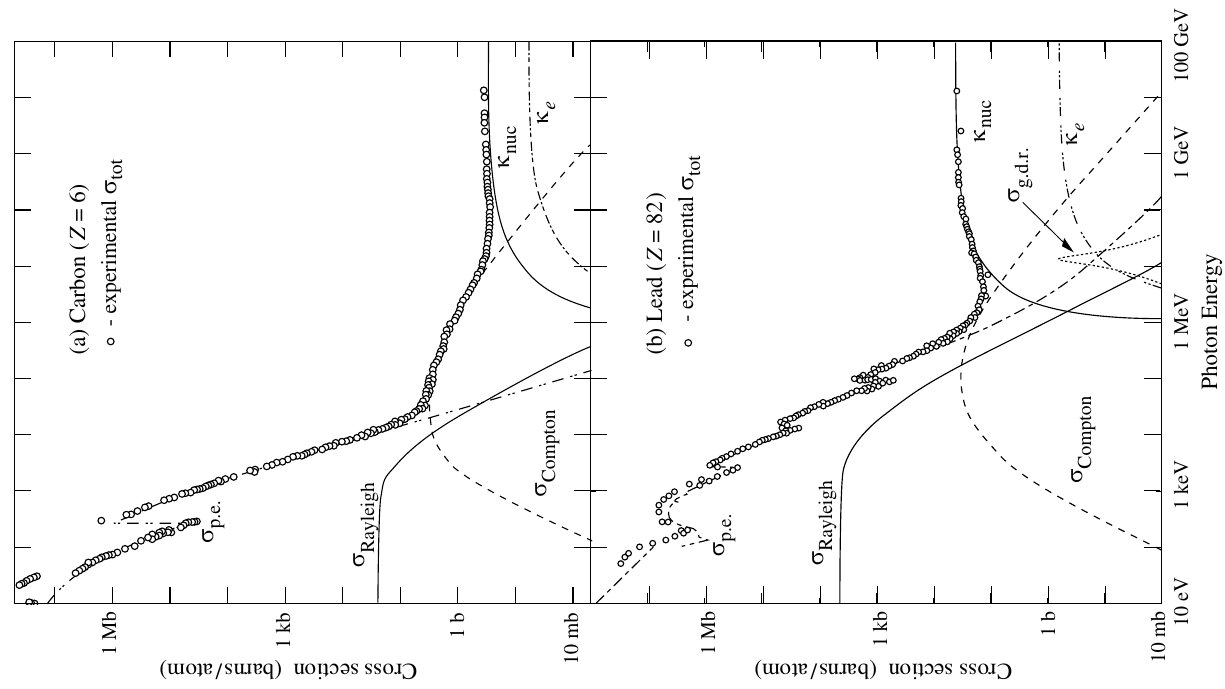
\includegraphics[width=1.2\linewidth,angle=270]{chap/description/fig/photon_energyloss}
	\caption{光子与物质各种相互作用的反应截面,上图是在碳中的,下图是在铅中的,引自\parencite{pdg_book}。}
	\label{fig:description:photon_energyloss}
\end{figure}

光子可以与物质发生多种相互作用,如图\ref{fig:description:photon_energyloss}所示。
其中${\sigma}_{p.e.}$是光电效应的反应截面,
${\sigma}_{Rayleigh}$是Rayleigh散射的反应截面, 
${\sigma}_{Compton}$是康普顿散射的反应截面,
${\kappa}_{nuc}$是靶核电场导致的电子对效应的反应截面,
${\kappa}_e$是靶核核外电子电场导致的电子对效应的反应截面,
${\sigma}_{g.d.r}$是光致核反应的反应截面。
在光子能量较低时光电效应占主导作用,中等能量时康普顿散射占主导作用,而高能光子一般只通过电子对效应损失能量.
从图\ref{fig:description:photon_energyloss}中可以看到电子对效应的反应截面非常小,再加上塑料闪烁体材料密度小、厚度薄,高能$\gamma$射线在PSD中发生反应的概率非常小,因此基本不会有能量沉积。

对于电子/正电子来说,它们的质量较小,在物质中的能量损失情况与重带电粒子有很大的不同。
电子/正电子与靶原子的相互作用,主要是电离能量损失,辐射能量损失和多次散射。
在能量较低时,电子/正电子虽然可以通过Møller散射,Bhabha散射和正电子湮灭损失能量,但电离能损仍然占据主导地位,见图\ref{fig:description:electron_energyloss}。
随着电子/正电子能量的升高,轫致辐射效应开始显著起来,并随着能量的增大近似以线性形式增强。
电离能损随着能量的增大以对数形式增强,因此当能量大于\SI{100}{MeV}之后轫致辐射导致的能损开始占据主导地位。
在DAMPE关注的能区,穿过PSD的电子/正电子主要通过轫致辐射损失能量。
然而,高能电子/正电子轫致辐射产生的光子能量也比较高,如前所述,它们一般不在PSD中沉积能量。
另一方面,电离相互作用虽然不占据主导作用,但它是一个连续过程,会一直在PSD中沉积能量,其大小大概与MIPs粒子的能量沉积差不多。

\begin{figure}[h!]
\centering
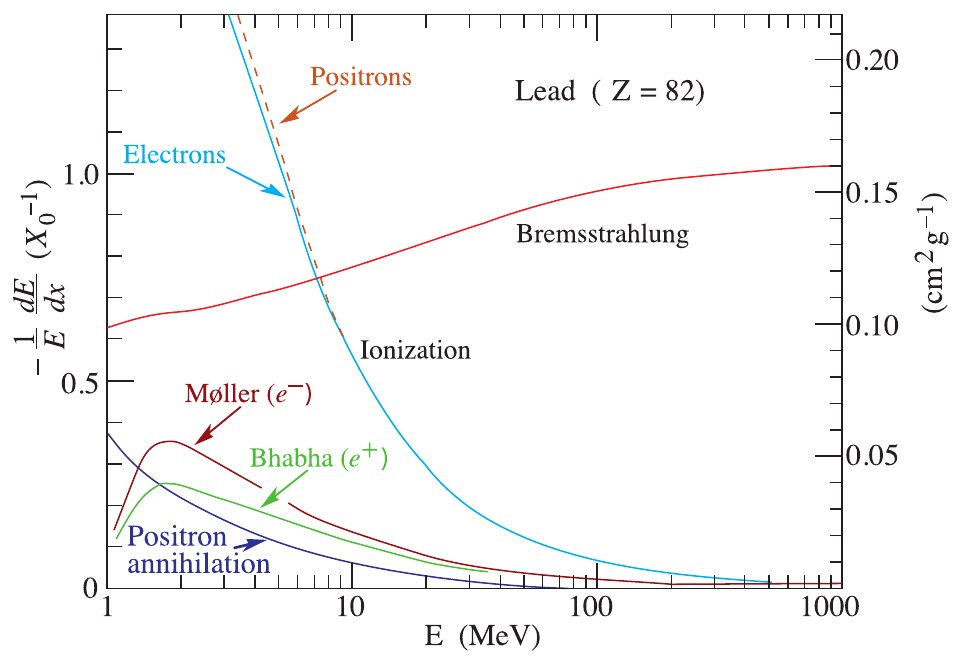
\includegraphics[width=0.8\linewidth]{chap/description/fig/electron_energyloss}
\caption{电子/正电子在铅中的单位辐射长度能损比例与能量的关系,引自\parencite{pdg_book}。}
\label{fig:description:electron_energyloss}
\end{figure}

综上所述,高能光子在PSD中没有能量沉积,高能电子/正电子在PSD中有能量沉积。
根据入射粒子是否在PSD中有能量沉积,可以将光子和带电粒子区分开来;进一步结合BGO量能器,可以进一步将电子/正电子和其它带电的强子区分开来。

\subsection{PMT的工作原理}
PMT是一种真空光电器件,具有光电转换和电子倍增两个功能。
它一般由入射光窗,光阴极,电子光学系统(即聚焦极)、电子倍增器(即打拿极串列)以及阳极组成。
这些组成部件被玻璃(或金属)外壳封装在真空环境中,使得电子在其中的运动不受空气中原子分子的影响。
PMT的结构多种多样,而端窗型是其中最常用的一种(PSD也使用端窗型PMT),图\ref{fig:description:pmt_structure}给出了该类型PMT的内部结构和工作过程示意图。

\begin{figure}[h!]
\centering
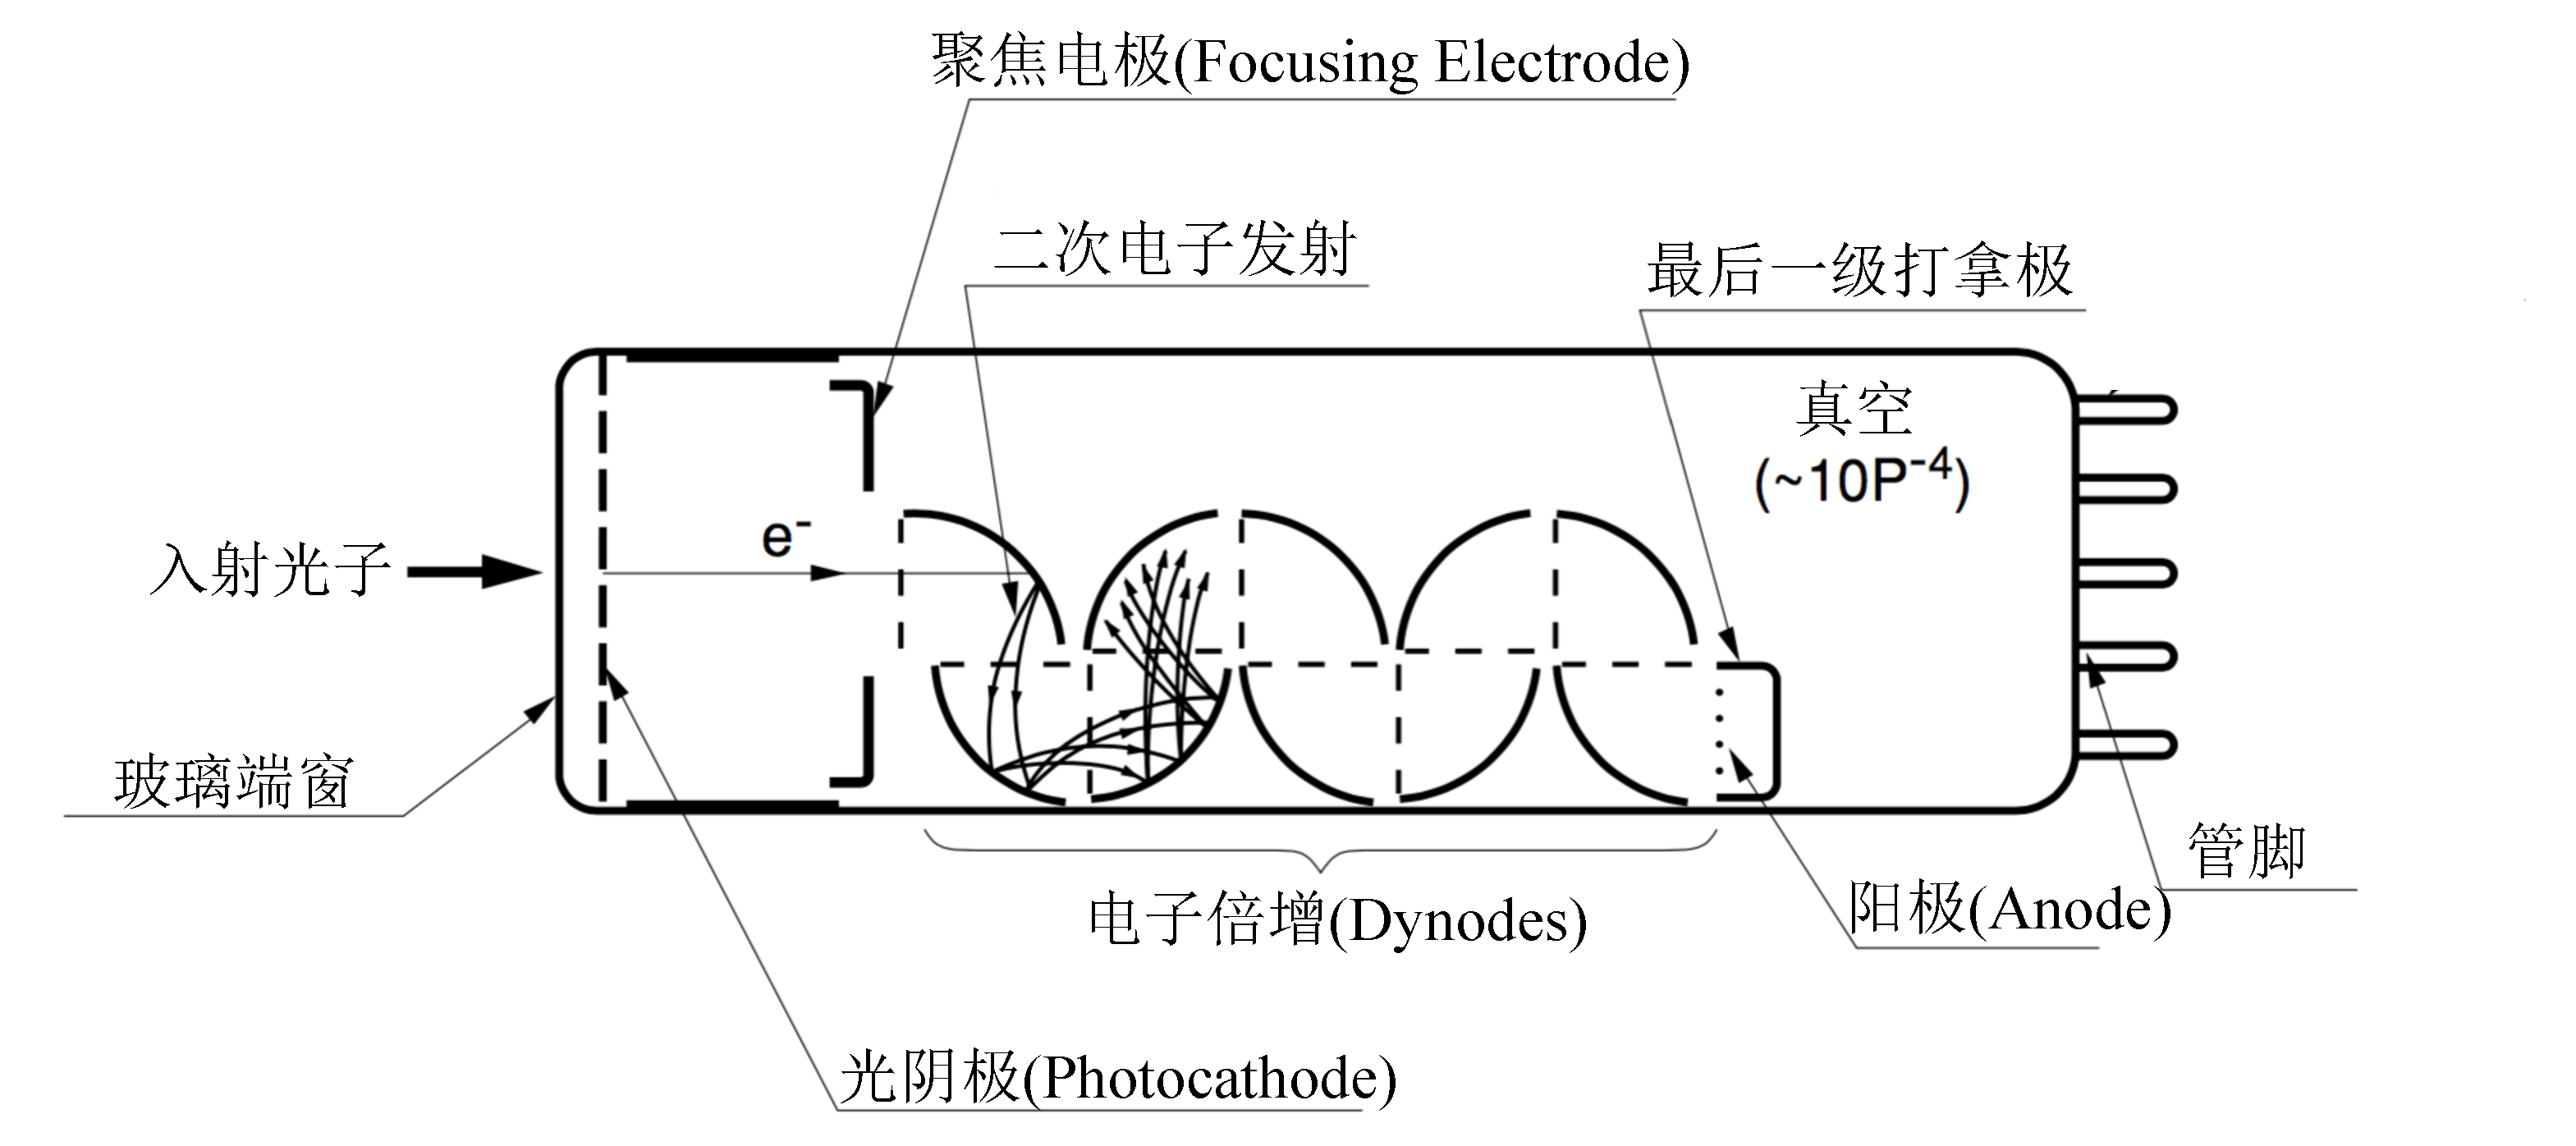
\includegraphics[width=\linewidth]{chap/description/fig/pmt_structure}
\caption{端窗型PMT的内部结构示意图}
\label{fig:description:pmt_structure}
\end{figure}

PMT工作时,需要在光阴极、聚焦极、各打拿极以及阳极间依次加上偏置高压,光阴极为负极性,阳极为正极性。
当没有光子入射时,PMT内部的电场分布呈稳定状态,各极间没有电流流动,即没有信号输出;
当有光子照射到入射光窗时,PMT按如下步骤产生电流信号:
\begin{enumerate}
	\item 光子透过玻璃端窗,击中覆盖在端窗内表面的光阴极材料。
	\item 通过光电效应(Photoelectric effect),光阴极内的电子被激发并逃逸到真空中。这部分逃逸电子被称为光电子。
	\item 在聚焦电极的加速、引导下,大部分光电子被聚焦,并击中第一打拿极。聚焦极和光阴极形成的电场能够控制电子的轨迹,因此它们也被称为电子光学系统。
	\item 打拿极材料一般使用二次电子发射系数($\delta\gg1$)较高的材料,这样一个原初电子轰击其表面就能产生$\delta$个次级电子。这些次级电子在极间电场的作用下,再次被加速并轰击下一个打拿极,从而产生更多的次级电子。多个打拿极串联在一起,使得电子逐级倍增,打拿极间的电流不断变大。这就是PMT的电子倍增过程,而打拿极串列也被称为PMT的电子倍增器。
	\item 最终,最后一个打拿极产生的次级电子被阳极收集并引出,倍增过程结束。%阳极也被称为收集极,为了最大化收集这些次级电子,阳极与最后一个打拿极的形状和布局一般不同于前面的打拿极串列。
\end{enumerate}
%这样,光信号在PMT内经过光电转换,聚焦,电子倍增和收集这一系列过程,最终被转换成了电流信号输出。

根据上述过程,PMT的阳极增益系数$G$可以表示为:
\begin{equation}
G = \frac{n_{anode}}{n_{photon}} = QE \times \eta \times M
\label{eq:description:pmt_gain}
\end{equation}
其中,$n_{anode}$是阳极输出的电子数目,$n_{photon}$是入射光子数目;
$QE$是光阴极的量子效率(Quantum Efficiency),它是光电子数与入射光子数的比值,表示光电效应的转换效率;
$\eta$是电子光学系统的收集效率(Collection Efficiency),它是第一打拿极收集到的电子数与光电子数的比值;
$M$是电子倍增器的增益系数,它是阳极输出的电子数与轰击第一打拿极的电子数的比值。

电子倍增器有多个打拿极串联组成,其增益系数$M$是各打拿极增益的乘积
\begin{equation}
M = \prod_{i=1}^{N} g_{i}
\label{eq:description:multiplier_gain}
\end{equation}
而打拿极增益$g_i$可进一步分解为
\begin{equation}
g_{i} = \eta_{i} \delta_{i}
\end{equation}
其中,$\eta_{i}$是第$i$打拿极到第$i+1$个打拿极间的电子收集效率 ,而$\delta_i$是第$i$打拿极的二次电子发射系数。
$\eta_{i}$和$\delta_i$都是极间电压$V_i$的幂函数,因此
\begin{equation}
g_{i} = k_i {V_i}^\alpha
\label{eq:description:dynode_power_function}
\end{equation}
$k_i$和$\alpha$都是常数,其中$k_i$与打拿极的几何结构有关,而$\alpha$与打拿极材料有关。
一般情况下,PMT的打拿极都使用相同的材料,因此$\alpha$对所有打拿极是一致的。
将公式\ref{eq:description:dynode_power_function}代入公式\ref{eq:description:multiplier_gain},同时考虑到极间电压是总电压$V_{ht}$固定的一部分($V_i=k^{'}V_{ht}$),可以得到
\begin{equation}
M = \prod_{i=1}^{N} k_i{V_i}^\alpha = \prod_{i=1}^{N} k_i{(k^{'}_i V_{ht})}^\alpha = KV_{ht}^{N\alpha}
\label{eq:description:multiplier_power_function}
\end{equation}
即PMT电子倍增器的增益系数是光阴极和阳极间所加总电压的幂函数。

量子效率$QE$是一个常数,它的值取决于所使用的光阴极材料,与所加电压无关。
电子光学系统的结构一般经过优化,其收集效率$\eta$虽然是电压的函数,但当光阴极和第一打拿极间的电压足够大时,可以认为$\eta\simeq1$。
基于这个假设,同时将公式\ref{eq:description:multiplier_power_function}代入公式\ref{eq:description:pmt_gain},可以得到PMT的整体增益也是所加总电压的幂函数
\begin{equation}
G = K^{'} V_{ht}^{{\alpha}^{'}}
\label{eq:description:pmt_gain_power_function}
\end{equation}
上式是光电倍增管的一个重要特性,它对PMT工作状态的调节具有指导意义,是PMT性能测试的主要内容。
PSD的PMT性能测试过程和结果将在第\ref{ch:pmt_test}章中进行详细叙述。


\section{探测器主体功能模块}

\subsection{PSD的整体构型}
\label{sec:description:psd_composition}
PSD采用模块化设计,它由多个探测单元模块组装成一个探测平面,且每个探测单元模块都能独立进行能量测量。
模块化设计带来两个好处:
\begin{itemize}
	\item 减小误判率。入射粒子在BGO量能器中发生电磁簇射或强子簇射时,大部分次级粒子都是前向的,但也有部分次级粒子由于大角度散射反照到PSD上。这些簇射次级粒子和原初入射粒子一样,在PSD上也会有能量沉积,这就可能造成光子被误判为带电粒子,或者质子被误判为重离子。PSD的模块化设计可以大大降低每个探测单元模块接收到的反散射粒子数,从而减少其对原初沉积能量的影响。实际使用中,首先通过STK重建的径迹反推出入射粒子击中的PSD探测单元,然后在根据该探测单元模块测得的沉积能量进行粒子鉴别和电荷测量,这样就能把反照粒子引起的PSD误判降到最低。
	\item 提供位置信息。PSD没有提取时间测量信息,因此不能使用常用的闪烁光到达两端的传播时间差方法对击中位置进行测量。PSD的位置信息来自击中探测单元的空间位置坐标,探测单元的宽度也就是PSD进行位置测量的最小单位。
\end{itemize}

\begin{figure}[htb]
	\centering
	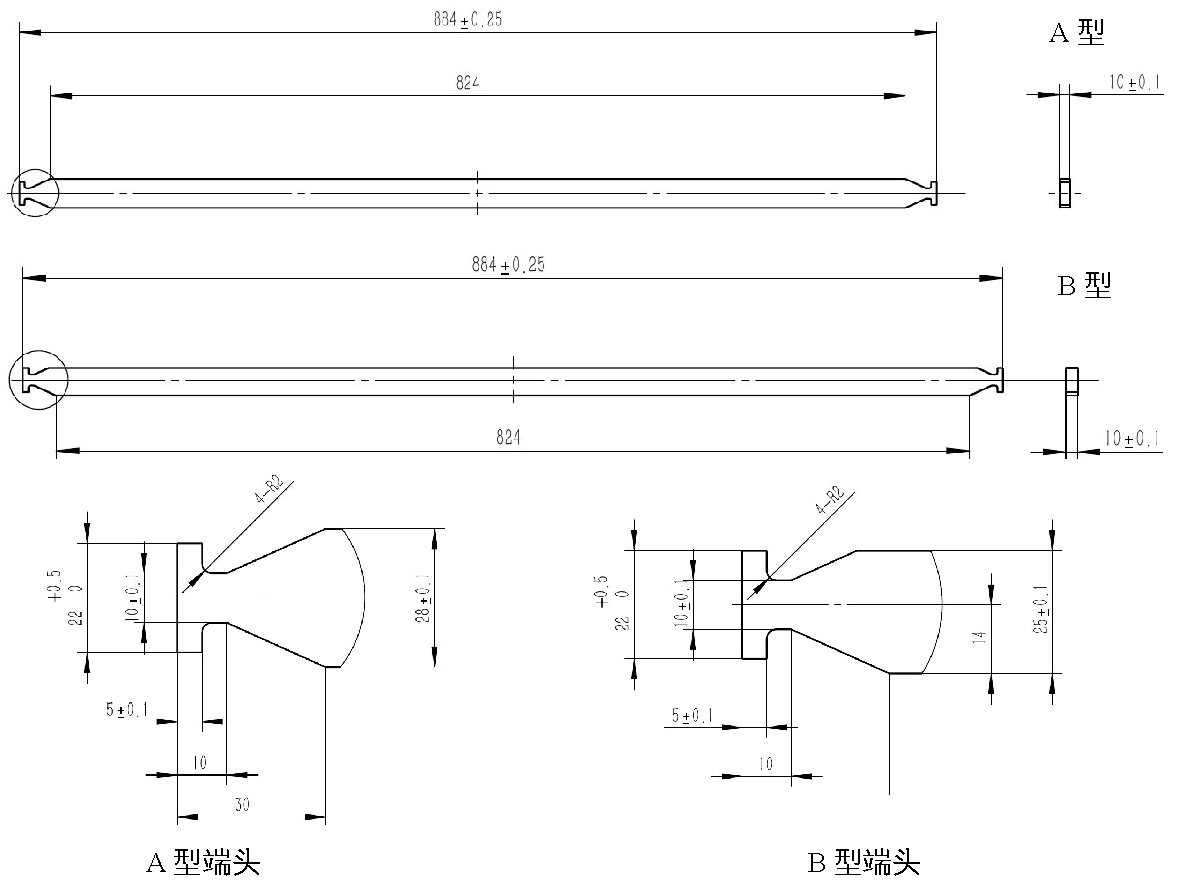
\includegraphics[width=\linewidth]{chap/description/fig/bars}
	\caption{PSD中两种塑闪单元条的尺寸}
	\label{fig:description:bars}
\end{figure}
PSD的最小探测单元是一根长度为\SI{884}{\milli\meter},厚度为\SI{10}{\milli\meter}的有机塑料闪烁体单元条。
单元条有A和B两种规格,分别对应两种宽度:A型宽度为\SI{28}{\milli\meter},B型宽度为\SI{25}{\milli\meter}。
图\ref{fig:description:bars}给出了这两种单元条的外形和具体尺寸信息。
可以看到,单元条的端头被加工成特殊的“工”字形,这是为了将单元条与支撑结构更好地固定在一起(详见第\ref{sec:description:psd_support}节)。
每根塑闪单元条的两端各耦合有一个光电倍增管作为读出器件,这就构成了PSD的一个探测器单元模块。

\begin{figure}[h!]
	\centering
	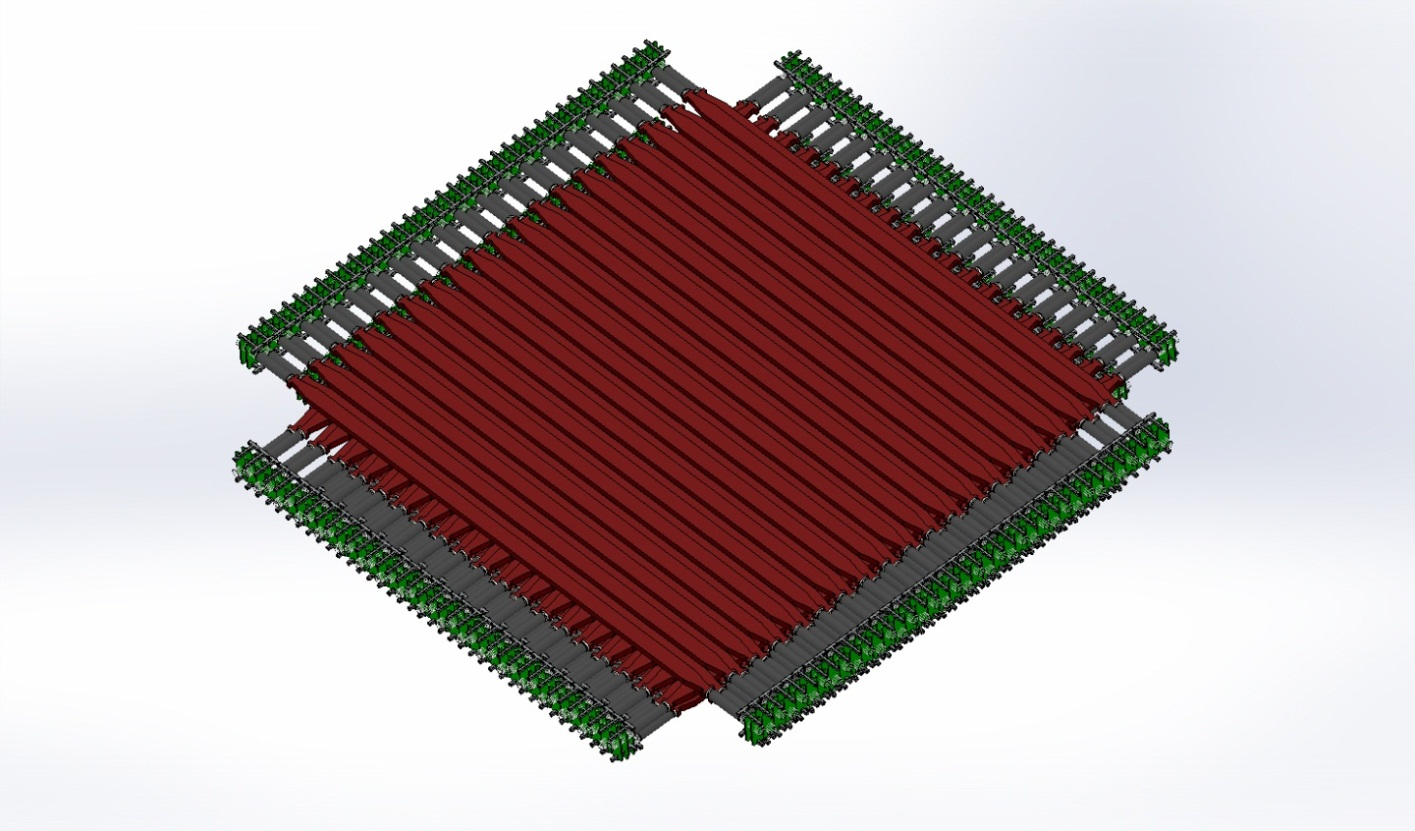
\includegraphics[width=0.72\linewidth]{chap/description/fig/psd_detector}
	\caption{PSD探测器的整体构型}
	\label{fig:description:psd_explosion}
\end{figure}

\begin{figure}[h!]
	\centering
	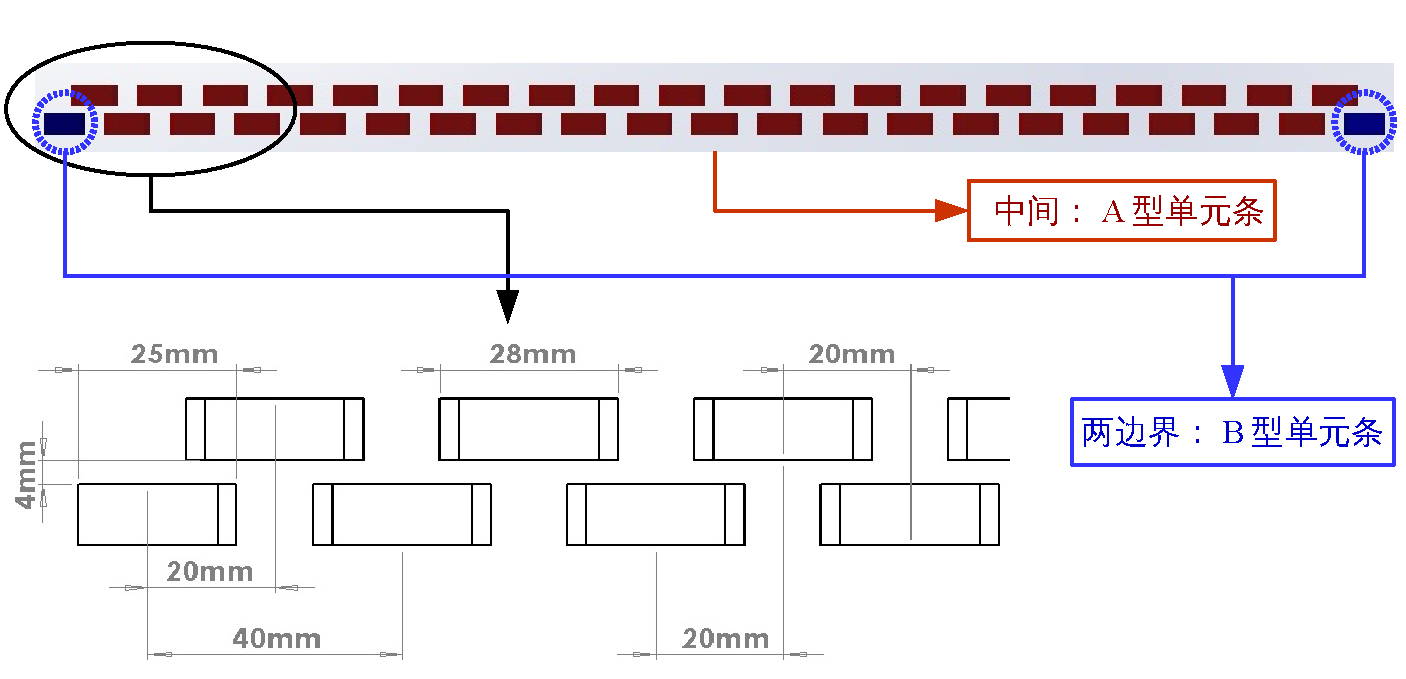
\includegraphics[width=0.8\linewidth]{chap/description/fig/bars_layout}
	\caption{塑闪阵列平面内的单元条交叠放置以消除探测器灵敏死区。}
	\label{fig:description:bars_layout}
\end{figure}

PSD一共由82个探测单元模块组成,分为X、Y两个相互垂直的塑闪阵列平面,如图\ref{fig:description:psd_explosion}所示。
两个探测平面的构型完全一样,由41个探测单元模块组成,其中39根A型单元条被放置在探测平面的中间部位,2根B型单元条分别被放置在探测平面的两个边界上。
在每个探测平面内,探测单元模块交错放置成“品”字形排列,以消除相邻单元条之间的间隙,见图\ref{fig:description:bars_layout}。
相邻探测单元模块的中心距离为\SI{20}{\milli\meter},因此单元条的重叠区域为\SI{8}{\milli\meter},足以消除DAMPE探测器广视角造成的探测器死区。
简单计算可以得到,PSD的有效探测面积为$\SI{822}{\milli\meter}\times\SI{822}{\milli\meter}$,并需要78根A型单元条,4根B型单元条以及164支PMT。

\subsection{探测器单元模块}
PSD选择了Eljen公司的EJ-200\parencite{ej-200}作为塑闪单元条材料,其主要性能参数参看表\ref{tab:description:ej200}。
EJ-200具有空间使用经验,曾被成功地使用到AMS-02项目中。
它具有良好的抗辐照性能,经过\SI{400}{\kilo\radian}剂量的辐照后,其性能不会发生明显的变化\parencite{ams02_tof}。
EJ-200本身具有较好的光传输性能,但由于PSD单元条的长度较长、宽度较窄,闪烁光子在单元条表面会发生多次反射和折射过程而损失掉。
为了提高光传输效率,PSD塑闪单元条的表面(除了与PMT耦合的端面)进行了抛光处理,同时使用Tyvek纸对塑闪单元条主体进行包装以提高反射率。
由于外部环境光会对PSD探测器单元模块的工作造成干扰,Tyvek包装层外又包裹了一层黑色热缩管材料进行避光,详见第\ref{ch:construction}章。

\begin{longtabu} to 0.8\linewidth{lX}
	\caption{EJ-200的主要性能参数\label{tab:description:ej200}}\\
	\toprule[1.5pt]
	\textbf{性能参数} & \textbf{典型值} \\ 
	\midrule
	\endfirsthead
	
	%\toprule[1.5pt]
	\multicolumn{2}{ c }{续表\ref{tab:description:ej200}}\\
	%性能参数 & 典型值 \\ 
	\midrule
	\endhead
	
	%\bottomrule[1.5pt]
	\endfoot
	
	\bottomrule[1.5pt]
	\endlastfoot
	
	H/C原子比 & 1.10 \\
	原子密度 & H: \SI{5.523E22}{\per\cubic\centi\meter}, C:\SI{4.740E22}{\per\cubic\centi\meter} \\
	光输出 & \SI{64}{\percent}(相对蒽)\footnote{\SI{60}{\celsius}时的光输出是\SI{20}{\celsius}时的\SI{95}{\percent},\SI{-60}{\celsius}$\sim$\SI{20}{\celsius}时光输出不依赖于温度} \\
	上升时间 & \SI{0.9}{\nano\second} \\
	衰减时间 & \SI{2.1}{\nano\second} \\
	光谱峰位 & \SI{425}{\nano\meter} \\
	衰减长度 & \SI{210}{\centi\meter} \\
	折射率   & 1.58 \\
	密度    &  \SI{1.032}{\g\per\cubic\centi\meter} \\
	膨胀系数 & \SI{7.8E-5}{\per\celsius} \\
	软化温度 & \SI{70}{\celsius} \\
	蒸气压   & 能用于真空 \\
	溶解性  &  可溶于芳香族溶剂、氯化溶剂及丙酮等,不溶于水、稀酸、低浓度酒精、碱及硅脂等 \\
\end{longtabu}

空间环境的特殊性对PMT的选择和使用提出了额外的要求,如力学性能(主要是火箭发射阶段的振动和冲击)和磁屏蔽性能(卫星磁棒以及地球的弱磁场)。
PSD选择了Hamamatsu公司的R4443-MOD2型光电倍增管作为读出器件,表\ref{tab:description:r4443}给出了它的具体性能参数。
\begin{figure}[htb]
\centering
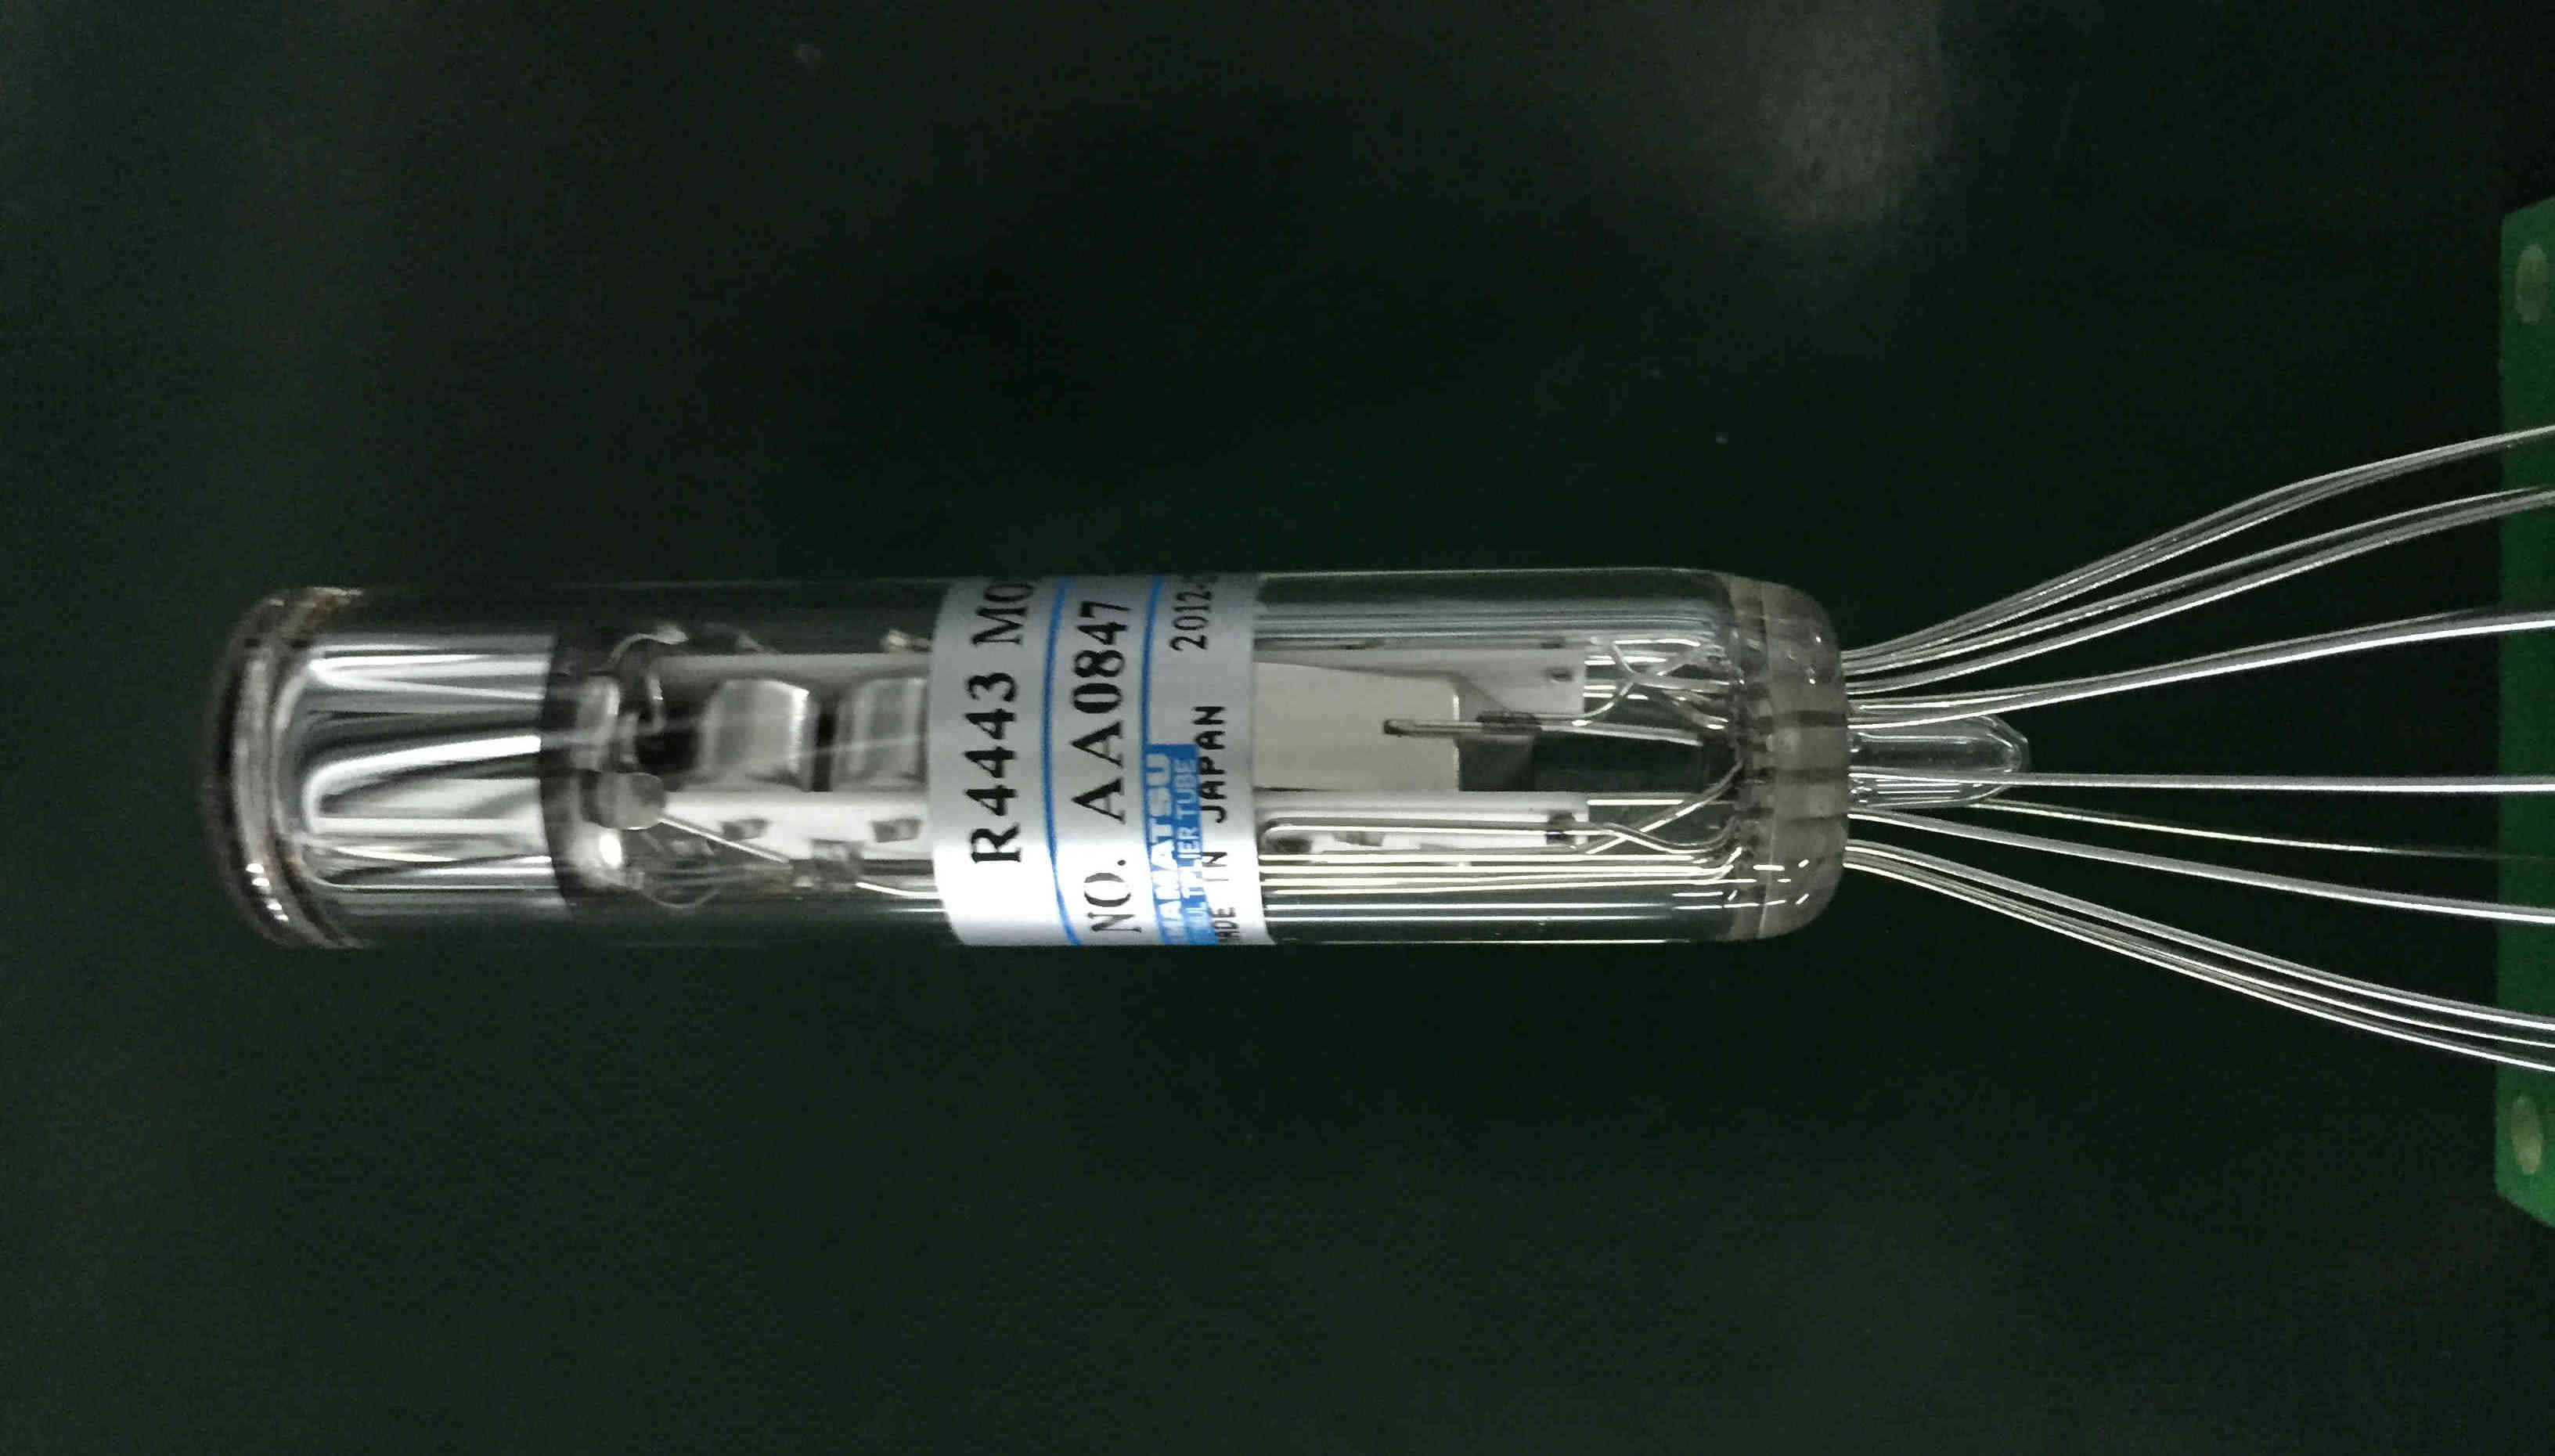
\includegraphics[width=0.6\textwidth]{chap/description/fig/r4443.jpg}
\caption{R4443-MOD2裸管}
\label{fig:description:r4443}
\end{figure}
R4443是一种端窗型、玻璃管身的光电倍增管(见图\ref{fig:description:r4443}),它的结构经过特殊的加固处理,能在恶劣的力学环境下工作;并且,R4443曾在FERMI-LAT项目上成功使用过,已有空间使用经历。
R4443-MOD2是R4443的升级版本,主要替换了光阴极材料,使得其暗电流大大降低。
它的基本结构没有改动,因此其力学性能可以得到保证。
根据模拟计算结果\parencite{psd_tdr},PSD探测器单元模块处的磁场强度小于\SI{5}{Gauss},因此R4443外部只需缠绕一层玻莫合金就可以屏蔽外部磁场对它的干扰。
为了提高可靠性,R4443外部灌封了硅胶保护层以进行力学减震,同时PMT整体将安装到一个铝合金保护套中并固定在探测器支撑结构上(详见第\ref{sec:description:psd_support}节)。
\begin{longtabu} to 0.6\linewidth{lX}
	\caption{R4443-MOD2的主要性能参数\label{tab:description:r4443}}\\
	\toprule[1.5pt]
	\textbf{性能参数} & \textbf{典型值} \\ 
	\midrule
	\endfirsthead
	
	%\toprule[1.5pt]
	\multicolumn{2}{ c }{续表\ref{tab:description:r4443}}\\
	%性能参数 & 典型值 \\ 
	\midrule
	\endhead
	
	%\bottomrule[1.5pt]
	\endfoot
	
	\bottomrule[1.5pt]
	\endlastfoot
	
	波长响应范围 & 300$\sim$650 \si{\nano\meter} \\
	光谱峰位 & \SI{375}{\nano\meter} \\
	光阴极材料 & 低噪声双碱金属 \\
	光阴极最小有效面积 & \SI{10}{\milli\meter} \\
	工作温度 & \SI{-30}{\celsius}$\sim$\SI{50}{\celsius} \\
	上升时间 & \SI{2.5}{\nano\second} \\
	渡越时间 & \SI{24}{\nano\second} \\
	打拿极数 & 10 \\
	典型增益 & \SI{1.0E6}{} \\
	最大工作电压 & \SI{1250}{\volt}\\
	重量 & \SI{11}{\g}\\
	外部尺寸(直径) & \num[separate-uncertainty]{14.5(7)} \si{\milli\meter} \\
	典型暗电流 & \SI{0.5}{\nano\ampere}\\
	最大暗电流 & \SI{4.0}{\nano\ampere} \\
	冲击 & \SI{5000}{\meter\per\square\second}(500 g's)\\
	振动 & \SI{200}{\meter\per\square\second}(20 g's) \\ 
\end{longtabu}

塑闪单元条与R4443之间使用硅脂垫片进行耦合。
硅脂垫片材料使用的是Eljen公司的EJ-560,其性能参数见表\ref{tab:description:ej560}。
EJ-560的折射率与R4443入射窗玻璃和塑料闪烁体的折射率非常接近,从而可以提高光耦合效率。
另外,硅脂垫片是一种弹性材料,使用它可以避免单元条与PMT之间的刚性接触,并释放塑闪单元条的温度形变产生的应力压迫,从而起到保护PMT的作用。
\newpage
\begin{longtabu} to 0.6\linewidth{lX}
	\caption{EJ-560主要性能参数\label{tab:description:ej560}}\\
	\toprule[1.5pt]
	\textbf{物理性能} & \textbf{典型值} \\ 
	\midrule
	\endfirsthead
	
	%\toprule[1.5pt]
	\multicolumn{2}{ c }{续表\ref{tab:description:ej560}}\\
	%性能参数 & 典型值 \\ 
	\midrule
	\endhead
	
	%\bottomrule[1.5pt]
	\endfoot
	
	\bottomrule[1.5pt]
	\endlastfoot
	
	厚度            & \SI{3}{\milli\meter}                      \\
	密度            & \SI{1.03}{\g\per\cubic\centi\meter}       \\
	硬度(A型邵氏硬度计)   & 16$\sim$24                           \\
	折射率           & 1.43                                      \\
	工作温度范围        & \SI{-40}{\celsius}$\sim$\SI{70}{\celsius} \\
	热膨胀系数         & \SI{3E-4}{\per\celsius}                   \\ 
\end{longtabu}

% \begin{table}[htb]
% 	\centering
% 	\caption{EJ-560主要性能参数}
% 	\label{tab:description:ej560}
	
% 	\begin{tabulary}{0.6\linewidth}{LC}
% 		\toprule[1.5pt]
% 		\textbf{物理性能} & \textbf{典型值}                              \\ 
% 		\midrule[1pt]
% 		厚度            & \SI{3}{\milli\meter}                      \\
% 		密度            & \SI{1.03}{\g\per\cubic\centi\meter}       \\
% 		硬度(A型邵氏硬度计)   & 16$\sim$24                                \\
% 		折射率           & 1.43                                      \\
% 		工作温度范围        & \SI{-40}{\celsius}$\sim$\SI{70}{\celsius} \\
% 		热膨胀系数         & \SI{3E-4}{\per\celsius}                   \\ 
% 		\bottomrule[1.5pt]
% 	\end{tabulary}
	
% \end{table}

\section{高压扇出功能模块}
\label{sec:description:psd_hv}
PSD探测单元模块的PMT高压由DAMPE的高压单机分系统提供。
由于卫星的资源限制,DAMPE高压单机不能给PSD的每个PMT提供独立的高压,多个PMT需要共享一个高压通道。
PSD高压扇出模块的功能就是将DAMPE高压单机提供的一路高压分为多路高压通道,并提供给各个PMT使用。

PSD的四个侧面各配备了一块高压扇出板,因此PSD一共需要4块高压扇出板。
每块高压扇出板上有6组高压分配电路,负责将来自DAMPE高压单机的6路输入高压按照$7+7+7+7+7+6$的模式提供给PSD一个侧面的41支PMT使用。
另外,DAMPE高压单机不能提供连续可调的高压值,只有8个高压档位可以使用,分别为\SI{0}{V}(小于\SI{60}{V})、\SI{780}{V}、\SI{810}{V}、\SI{840}{V}、\SI{870}{V}、\SI{900}{V}、\SI{930}{V}以及\SI{960}{\volt}。
这些限制条件要求PSD同一高压组别内的R4443需要有相似的增益和增益特性曲线,这个问题将在第\ref{ch:pmt_test}章和第\ref{ch:construction}章详细讨论。

\section{前端电子学功能模块}
\label{sec:description:psd_electronics}
前端电子学功能模块(Front-End Electronics,简称FEE)是PSD的数据处理单元,它接收来自DAMPE载荷数管机箱分系统的控制信号和触发信号,产生PSD的科学数据、工程参数数据以及遥测数据,并传输到载荷数管机箱分系统中。
载荷数管是DAMPE探测器的数据处理中心,它负责与卫星的通信并协同各子探测器间的工作;来自子探测器的数据在载荷数管进行重组并被发送到载荷管理器的存储单元,等待卫星入站后由数传通道下行到地面。

\begin{figure}[htb]
	\centering
	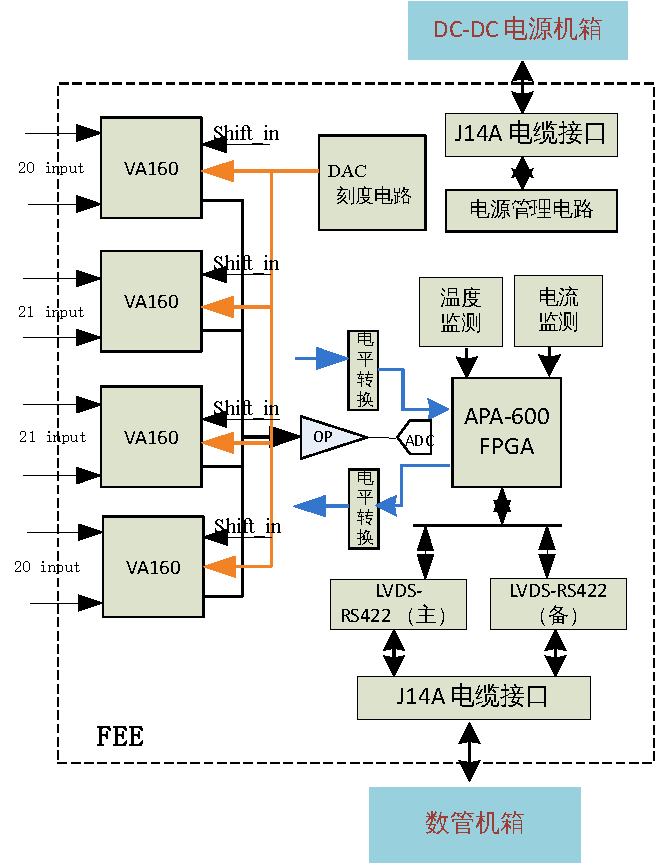
\includegraphics[width=0.7\linewidth]{chap/description/fig/psd_fee1}
	\caption{PSD的前端电子学原理框图。}
	\label{fig:description:psd_fee1}
\end{figure}
PSD的前端电子学功能模块一共由4块前端电子学板(简称FEE板)组成,每个侧面一块,负责该面41支PMT信号的处理。
图\ref{fig:description:psd_fee1}给出了FEE板的原理框图,它由以下功能电路组成:钳位保护电路、电荷测量电路、模拟调理电路、模数变换电路、刻度电路、温度/电流监测电路、FPGA、电源管理电路以及接口电路。
下面,对FEE板的主要功能做一个简单介绍,FEE的详细设计可以参看文献\parencite{yanghaibo_thesis,psd_tdr}。

\subsection{电荷测量}
电荷测量是FEE板最重要的功能之一。
PSD选择了一款来自挪威IDEAS公司的ASIC(Application Specific  Integrating Circuit)芯片作为电荷测量的核心电路。
VA160是一款高集成度、低功耗、高灵敏度的电荷测量芯片,能够满足DAMPE卫星对载荷的功耗、空间和重量限制,表\ref{tab:description:va160}给出了VA160的主要性能参数。
VA160是VA32的改进版本,而VA32在AMS-02项目中成功使用过,因此其空间抗辐照性能也可以得到保证。
\begin{table}[h]
	\centering
	\caption{VA160的主要性能参数}
	\label{tab:description:va160}
	
	\begin{tabulary}{0.8\linewidth}{Ll}
		\toprule[1.5pt]
		\textbf{参数} &                     \textbf{典型值}                       \\ 
		\midrule[1pt]
		通道数         &                          32                            \\
		电荷测量范围      &           \SIrange{-3}{13}{\pico\coulomb}            \\
		成形时间        &          \SIrange{1.8}{2.3}{\micro\second}            \\
		等效噪声电荷(ENC) &       3200 \si{e} + 7.6 \si{e\per\pico\farad}          \\
		积分非线性       &                   \SI{2}{\percent}                     \\
		功耗          & 平稳工作:\SI{181}{\milli\watt},最大值:\SI{203}{\milli\watt}   \\ 
		\bottomrule[1.5pt]
	\end{tabulary}
\end{table}

\begin{figure}[htb]
	\centering
	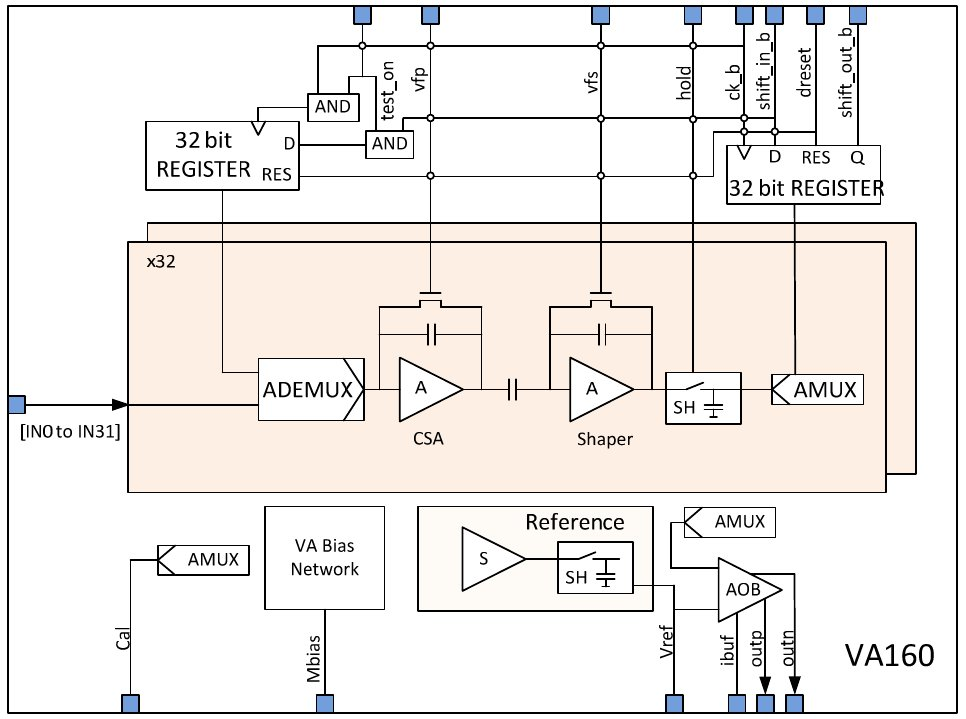
\includegraphics[width=0.8\linewidth]{chap/description/fig/va160}
	\caption{VA160原理框图,引自\parencite{fengchangqing_eqm}}
	\label{fig:description:va160}
\end{figure}

图\ref{fig:description:va160}是VA160的电路原理框图。
VA160一共有32个独立的电荷测量通道,每个测量通道都是一个完整的电荷测量电路,包括:电荷灵敏前置放大器(CSA),CR-RC成形电路(Shaper)和采样保持电路(SH)。
VA160采用电流-电荷方法进行电荷测量:来自R4443的电流脉冲信号通过钳位保护电路直接输入到VA160中;前置放大器对输入的电流脉冲进行积分,并输出与电荷量成正比的电压;电压信号之后经耦合电容输入到成形电路中,成形后的准高斯波形在$\sim$\SI{1.8}{\micro\second}处到达峰值,且峰值大小与输入电压成正比;最后,采样保持电路在某个时刻产生一个保持信号,并将成形电路此时刻的输出电压保持住以等待后续电路的处理。
为了能够准确测量输入的电荷量,保持信号应该在成形脉冲到达峰值时产生,这样才能采到峰值电压,如图\ref{fig:description:sample_hold}所示。
由于成形时间在微秒量级,DAMPE的触发信号一般在达峰之前到来,因此保持信号需要在触发信号延迟一段时间后产生。
所有测量通道最终通过一个32选1的模拟多路开关依次经过电流输出型全差分放大器输出。
VA160输出的差分电流信号经过模拟调理电路后被转换成电压信号,最后输入到一款14位的高精度ADC中进行模/数转换并被记录下来。
除了32个正常的测量通道外,VA160内还有一个悬空参考通道,用于抑制共模噪声和由温度引起的电子学漂移。

\begin{figure}[h!]	
	\centering
	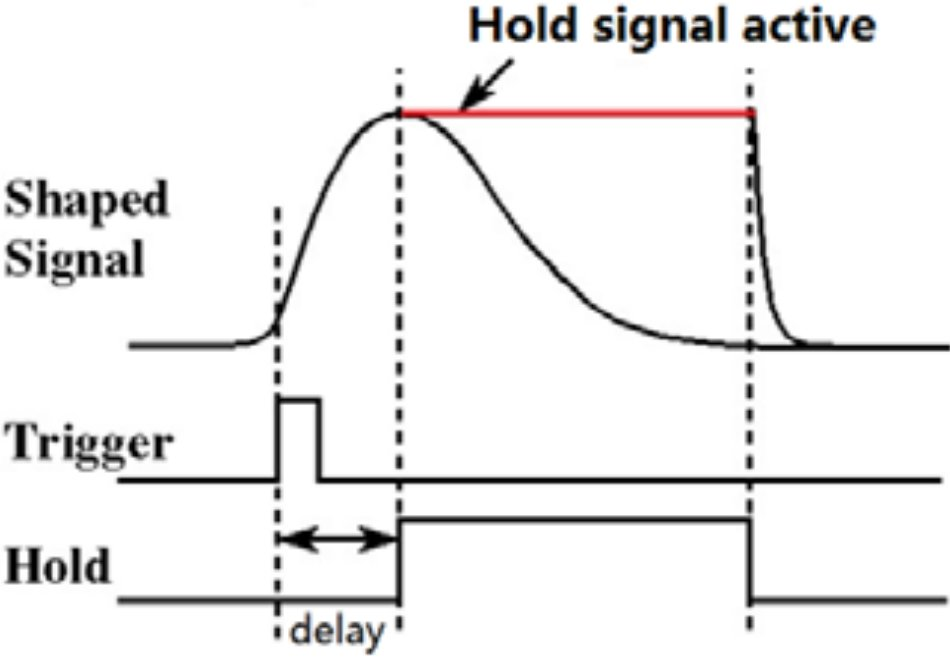
\includegraphics[width=0.5\linewidth]{chap/description/fig/sample_hold}
	\caption{保持信号与触发信号的关系。}
	\label{fig:description:sample_hold}
\end{figure}

PSD的每个侧面有41支PMT,每支PMT输出两个信号(双打拿极读出设计,详见第\ref{ch:large_dynmaicrange}章),因此每个侧面一共有82个待测电流信号。
由于两个打拿极的信号幅度相差较大,为了减少通道间的串扰,来自不同打拿极的信号被连接到不同的VA160芯片上。
因此,每块FEE板上使用了4片VA160芯片。
另外,除了真实信号通道外,每片VA160上还额外引出2个悬空通道(冗余设计)用于监测电子学噪声,最终每块FEE板会记录90个通道的科学数据。

\subsection{电子学刻度}
电子学刻度指的是:利用电荷量已知的脉冲信号模拟真实的PMT输入信号,对FEE每个测量通道的性能进行标定和自检。
PSD设计了专门的电子学刻度电路,并集成在FEE板上,它具有如下几个功能:
\begin{enumerate}
	\item 为了准确测量信号电荷量,FEE的电荷测量电路(包括VA160测量通道、模拟调节电路和模/数转换)需要具有良好的线性。通过电子学刻度可以得到整个电子学测量通路的线性范围,同时得到非线性参数,以便对结果进行离线修正。
	\item 在调试、运行过程中,通过了解FEE电荷测量通道的性能状态,可以发现异常状况和故障,因此电子学刻度电路兼具自检的功能。
	\item DAMPE卫星的设计寿命是3年,长时间的运行过程中,工作环境、器件老化等因素会引起电荷测量电路的参数变化。通过电子学刻度对各测量通道进行定期的标定,可以监测并修正这些参数变化,保证测量结果准确有效。
\end{enumerate}

电子学刻度的信号产生电路由模拟开关(Switch)、参考电平产生电路(DAC)、放电电阻(\SI{10}{\kilo\ohm})以及刻度电容($C_{calib}$=\SI{10}{\pico\farad})组成。
图\ref{fig:description:fee_calibration}给出了PSD电子学刻度电路的原理图。
DAC输出一个恒定的参考电压$V_{ref}$,FPGA控制模拟开关的通断从而产生一个阶越的电压信号。
此时,为了使得刻度电容的电压值达到参考电压值$V_{ref}$,刻度电容两端会产生一个脉冲电流对刻度电容充电。
由于刻度电容左端与VA160的Cali管脚相连,因此这个脉冲电流被直接用于VA160的通道刻度,其对应的电荷量为$Q_{calib}=V_{ref}C_{calib}$。
通过改变DAC的输出电压值,可以得到一系列不同电荷量大小的脉冲电流,从而对测量通道进行电荷扫描,得到其线性曲线。

\begin{figure}[h!]
\centering
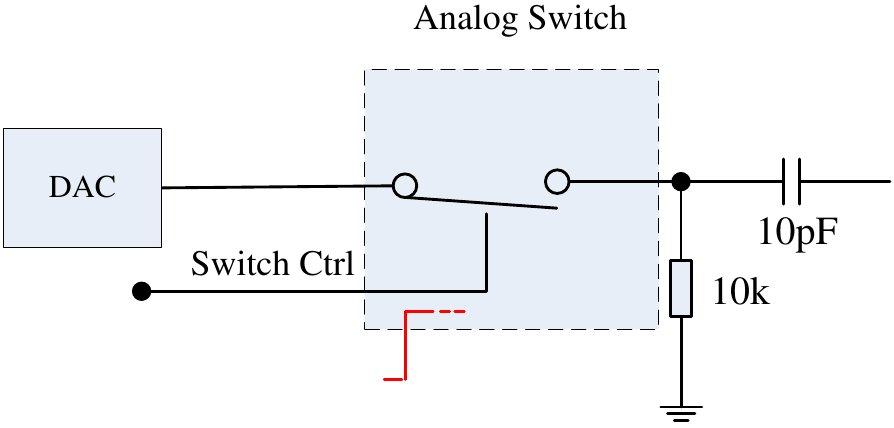
\includegraphics[width=0.7\linewidth]{chap/description/fig/fee_calibration}
\caption{电子学刻度电路原理}
\label{fig:description:fee_calibration}
\end{figure}


\subsection{温度/电流监测}
PSD的工作温度范围为\SI{-10}{\celsius}$\sim$\SI{30}{\celsius}。在这么大的温差范围内,探测器部件(PMT和塑闪单元条)以及电子学器件的温度效应会对探测器的性能造成影响。
因此,PSD在探测器内部以及FEE板上多个位置放置了热敏电阻,以对环境温度进行监测。
温度测量值最终通过FEE板上的ADC转化为数字量,并传输到载荷数管。
数据分析时,根据温度测量电路测得的环境温度值,可以对上述温度效应进行修正。

空间中,单个带电粒子入射产生的瞬态电流触发CMOS器件中可控硅结构使其导通,由于可控硅的正反馈特性使电流不断增大,进入大电流再生状态,即导致锁定,这种现象被称为单粒子锁定(Single Event Latchup)。
单粒子锁定导致电流变大,局部温度升高;重新掉电、上电可以清除单粒子锁定,但如果没有迅速断电,过度的加热可能会造成器件的永久性损坏。
VA160是PSD最重要的功能器件,电流监测电路主要用于监测VA160是否发生单粒子锁定。
FEE采用电流采样电阻+ADC的方式监测VA160的-2.5V直流电源电压的电流,载荷数管会定时(1 次/秒)收集各FEE的电流值,如果连续3次发现该电流值超标,载荷数管应立即把该FEE对应侧面的PMT高压降到低压档位,1秒钟后对DC-DC电源机箱发送相应断电指令,使该侧面的FEE关机,以保护FEE。


\section{机械支撑功能模块}
\label{sec:description:psd_support}
PSD的探测器主体功能模块、前端电子学功能模块和高压扇出功能模块都安装在机械支撑功能模块中。
PSD的机械结构能够稳固地支撑各内部组件,同时减缓火箭升空过程中的机械冲击和振动,保护脆弱部件不受损伤,保证PSD的功能完整性。

\begin{figure}[h!]
	\centering
	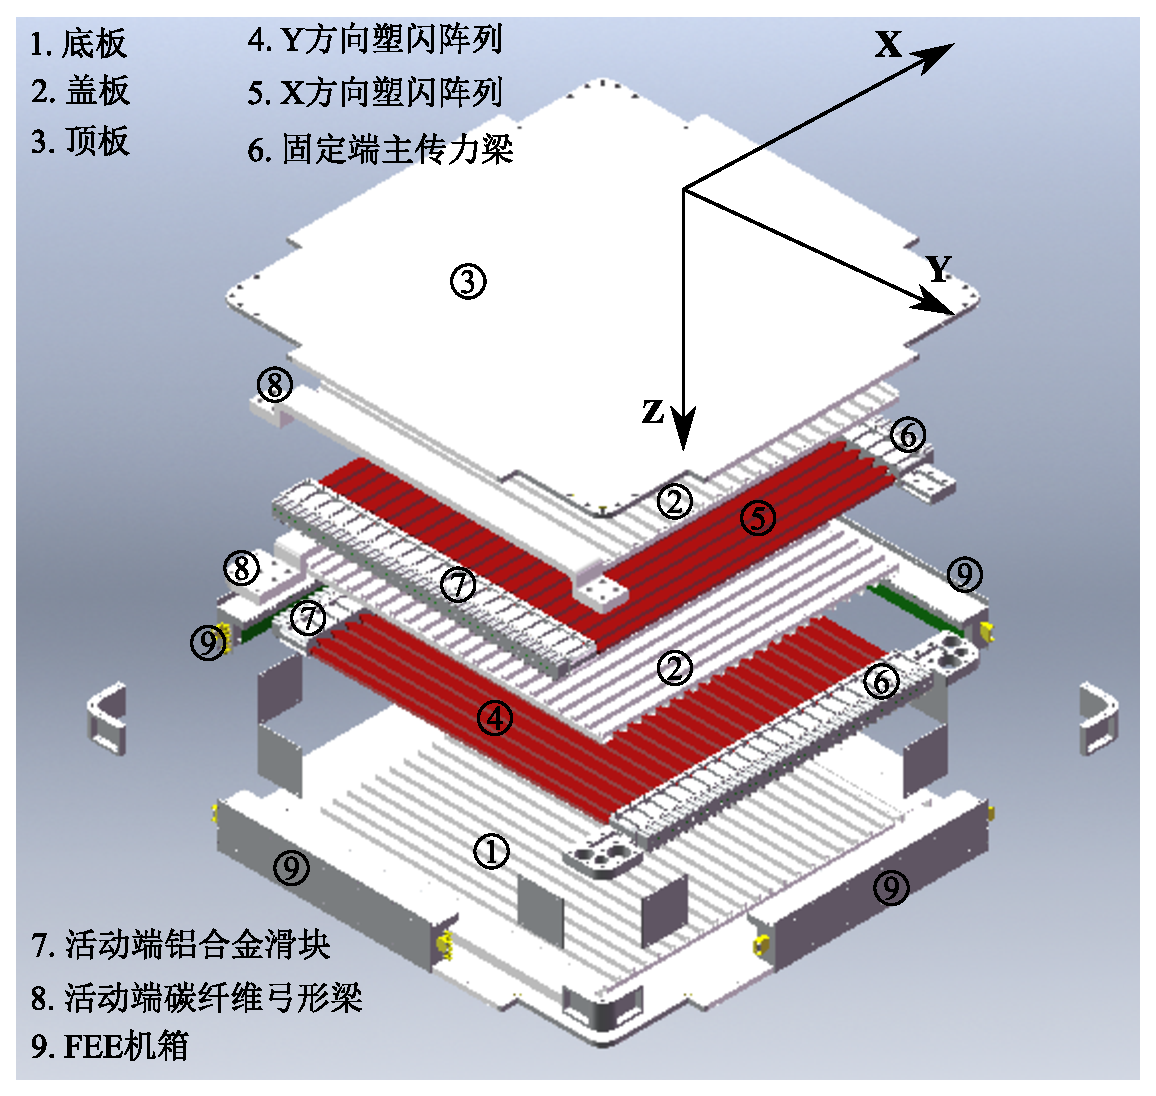
\includegraphics[width=0.8\linewidth]{chap/description/fig/psd_explosion.eps}
	\caption{PSD结构的爆炸图展示}
	\label{fig:description:psd_structure}
\end{figure}

图\ref*{fig:description:psd_structure}给出了PSD整体结构的爆炸图展示。
底板和顶板,加上四个角上的连接法兰以及四个侧面的FEE机箱构成了PSD的主体包络($\SI{1200}{\milli\meter}\times\SI{1200}{\milli\meter}\times\SI{126}{\milli\meter}$)。
整个外包络组成一个封闭的内部空间,能够有效抵挡外部太阳光的照射,使得内部的PMT和塑闪单元条免受外部杂散光线的影响。
为了减轻重量和减少探测器灵敏面积内的物质量,底板和顶板采用碳纤维蒙皮的铝蜂窝板结构,并在四周主要承力部位预埋碳纤维方管和铝合金榫头组成的框架以加强刚度和强度。
连接法兰用于连接顶板和底板主传力结构,它采用铝合金材料。
FEE机箱内安装有该侧面对应的FEE前端电子学板、高压扇出板和信号转接板。
考虑到箱体结构的力学性能,FEE机箱的主体结构由铝合金整体铣制加工而成。
FEE机箱的侧板和顶板同样由铝合金材料加工而成,并与主箱体无缝衔接以提高电磁屏能力和导热性能。

PSD的主承力结构由4组梁结构和底板连接为一个整体组成,主要用于固定和保护塑闪单元条阵列及其PMT组件,见图\ref{fig:description:bottom_plate}。
底板中间的凸台上具有由由碳纤维方管隔断的凹槽结构,槽体近似与塑闪单元条等宽,用于保护塑闪单元条。
每根梁的主体由三层铝合金组件构成, 其内部具有两排(一排21个,一排20个)“工”字形和圆柱形组成的凹槽结构,用于固定41个塑闪单元模块的一端。
“工”字形凹槽与塑闪单元条的“工”字形端头适配,用于固定塑闪单元条;圆柱形孔结构紧连“工”字形槽结构,用于安装PMT组件。
图\ref{fig:description:pmt_protection}给出了PMT组件安装在PSD结构上的示意图。
\begin{figure}[h!]
\centering
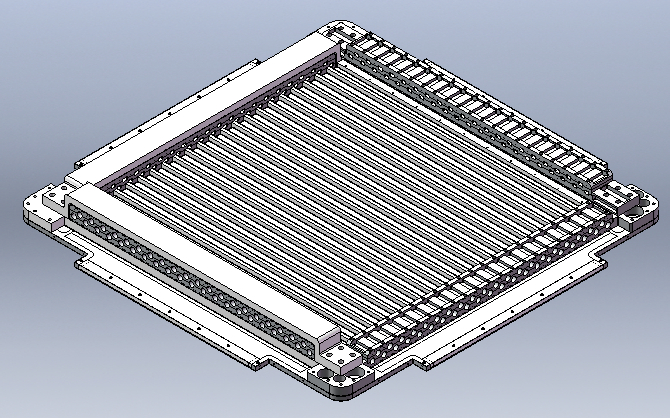
\includegraphics[width=0.7\linewidth]{chap/description/fig/bottom_plate}
\caption{PSD主承力结构}
\label{fig:description:bottom_plate}
\end{figure}

\begin{figure}[htbp]
	\centering
	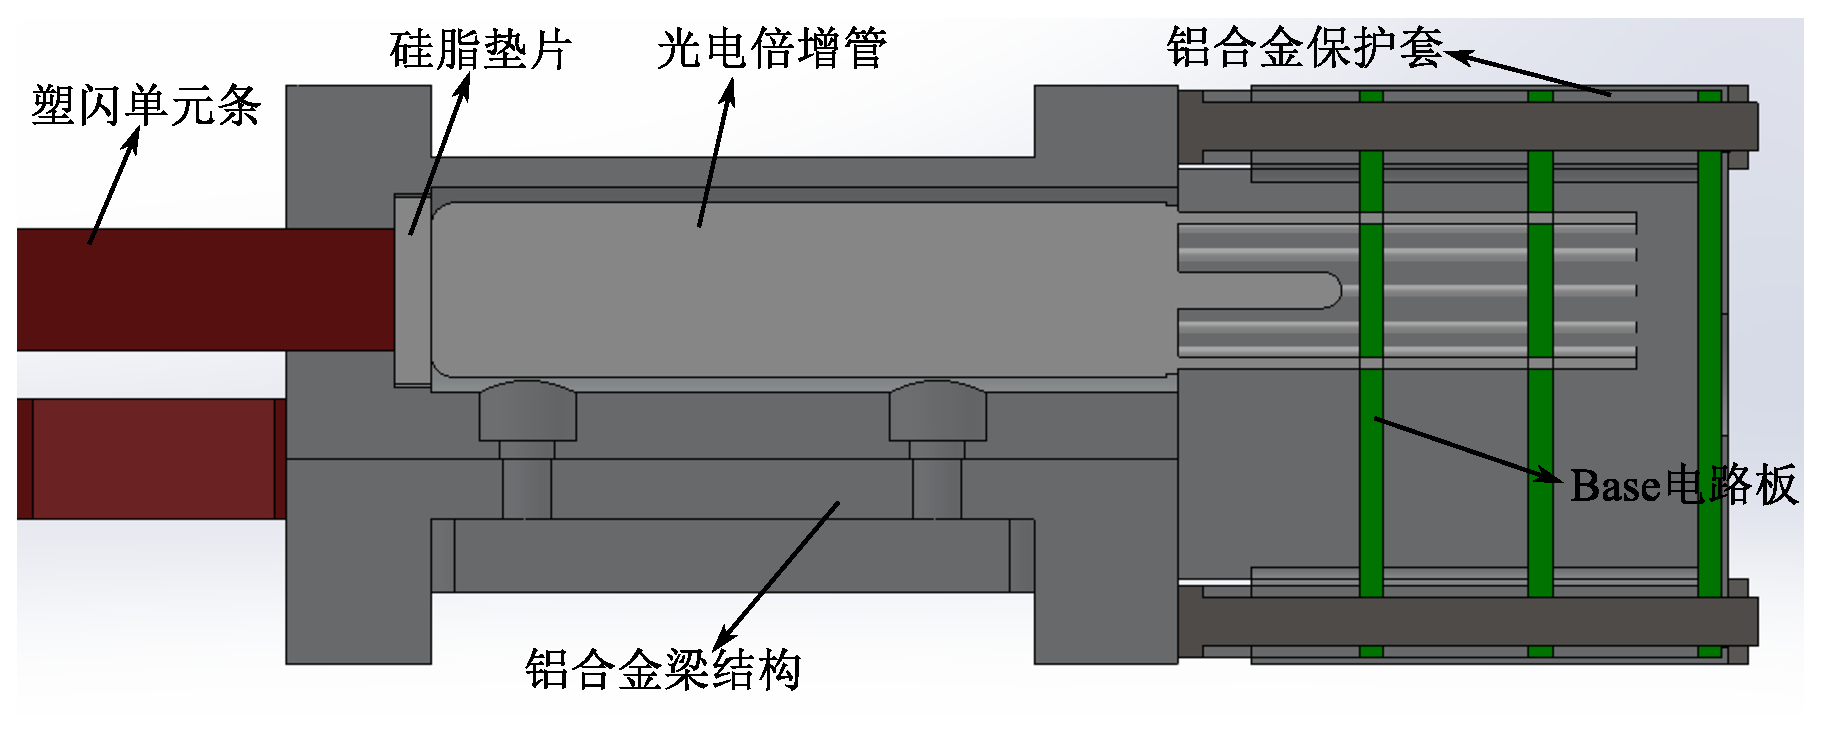
\includegraphics[width=0.8\textwidth]{chap/description/fig/pmt_protection.eps}
	\caption{PMT的安装示意图}
	\label{fig:description:pmt_protection}
\end{figure}

每个塑闪阵列平面由两组梁结构固定,并被分为固定端和活动端,见图\ref{fig:description:girders}。
固定端梁只由三层铝合金组件组成,下层铝合金较其余两层稍长并直接与碳纤维底板连接,完全约束了单元条固定端的6个自由度。
活动端梁由三层铝合金组件和一个碳纤维弓形梁组成。三层铝合金组件自身连接成一个整体,该结构不和底板连接,被称为铝合金滑块;碳纤维弓形梁与铝合金滑块外形完全适配并与底板直接连接,它和底板组成梁结构完全约束单元条活动端的5个自由度,底板和铝合金滑块间的摩擦力约束了沿塑闪单元条长度方向的自由度。
当温度变化时,塑闪单元条变形力能够克服摩擦力,并带动铝合金滑块小范围来回滑动从而释放塑闪单元条形变,保证单元条不因膨胀收缩而断裂。

\begin{figure}[h!]
	\centering
	\subfloat[][固定端铝合金滑块]{
		\label{fig:description:fixed_girder}
		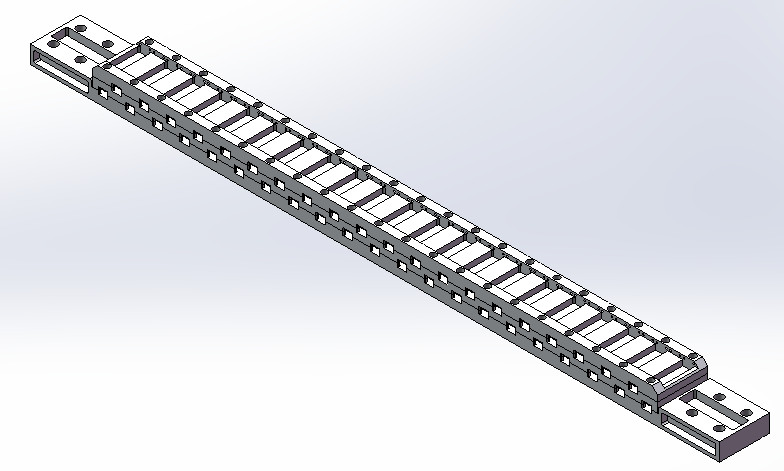
\includegraphics[width=80mm]{chap/description/fig/fixed_girder}
	}
	\subfloat[][活动端铝合金滑块]{
		\label{fig:description:moving_girder}
		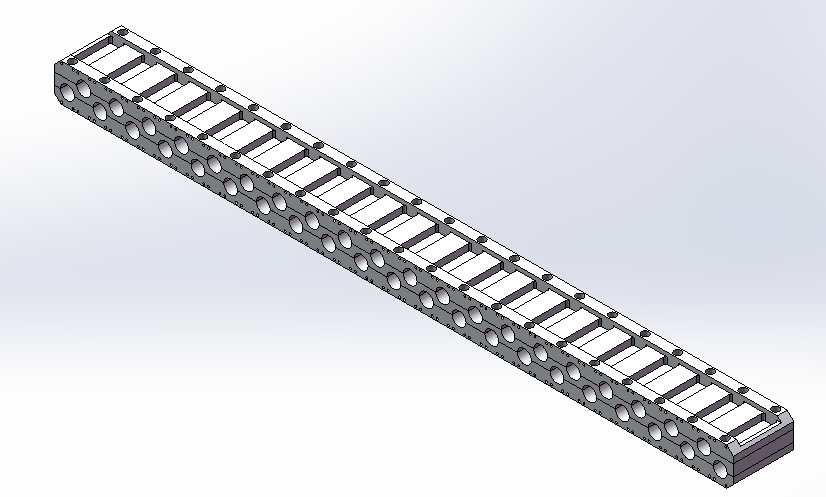
\includegraphics[width=80mm]{chap/description/fig/moving_girder}		
	}
	\caption{铝合金滑块}
	\label{fig:description:girders}
\end{figure}

最后,两个塑闪阵列平面间以及上层塑闪阵列平面与顶板间还各有一块碳纤维盖板,用于保护塑闪单元条。

\section{主要技术指标与关键技术、工艺}
\label{sec:description:psd_requirements}
\subsection{主要性能指标}
根据DAMPE粒子探测器整体的物理需求,PSD需要满足如下性能指标:
\begin{enumerate}[noitemsep,topsep=0pt]
	\item 有效探测面积$\SI{820}{\milli\meter}\times\SI{820}{\milli\meter}$。DAMPE是单方向的探测器,它只关心从顶部入射的粒子。由于PSD位于DAMPE探测器最顶端,它的有效探测面积决定了DAMPE的视场大小,因此PSD也是DAMPE中面积最大的子探测器系统。
	\item 探测单元模块实现电子和重离子($Z=1\sim20$)的沉积能量测量。根据\ref{sec:description:psd_principle}节的描述,不同入射粒子在PSD中的能量沉积相差巨大,这需要PSD的探测单元模块具有较大的读出动态范围。另外,为了有效区分电子信号和噪声本底(光子不在PSD中产生信号),探测单元模块还需要有较高的信噪比。PSD探测单元模块的读出设计将在第\ref{ch:large_dynmaicrange}章进行详细讨论。
	\item 探测单元模块的电荷分辨优于\SI{25}{\percent}。为了对重离子进行有效鉴别,探测器的能量分辨率需要满足一定条件。由于塑料闪烁体材料本身的限制,PSD探测单元模块的能量分辨率要求被确定为:对$Z=1$的粒子(对于$Z>1$的重离子,探测器响应很难在实验室条件下进行验证)好于\SI{25}{\percent}。
	在相对论能区,所有$Z=1$的粒子与MIPs粒子具有类似的能量沉积,因此这个要求可以转化为对MIPs粒子的能量分辨率好于\SI{25}{\percent}。
	\item 各探测单元模块的MIP能量响应一致性好于\SI{25}{\percent}。PSD的整体性能是各探测单元模块归一化的结果,不同单元之间较好的能量响应一致性有利于PSD整体性能的优化。
	\item 空间分辨好于\SI{2}{\centi\meter}。径迹探测并不是PSD的主要功能,DAMPE的主要径迹探测器是STK。但在径迹寻找和重建过程中,STK需要BGO和PSD提供的额外位置信息作为“种子”,同时PSD的位置信息也可以用于真实迳迹的验证。
	因此,PSD的位置信息不需要特别精确,其分辨率最终被确定为\SI{2}{\centi\meter}。
	\item 对MIPs粒子的探测效率高于\SI{95}{\percent}。
	这是$e/\gamma$鉴别提出的要求,它包含两部分内容:一是对带电粒子的探测器效率高于\SI{95}{\percent},二是对光子的误判率低于\SI{5}{\percent}。
\end{enumerate}

\subsection{关键工艺与技术}
塑闪单元条温度形变适应结构设计、探测单元模块大动态范围读出设计以及PMT组件灌封工艺是PSD的关键技术与重要工艺。
塑闪单元条温度形变适应通过PSD支撑结构上活动端与固定端梁组成的五维约束结构予以解决,详见\ref{sec:description:psd_support}节。
在PSD的方案阶段,该结构设计的可行性和合理性通过软件仿真分析、模拟件试验以及结构件的高低温试验得到了充分的验证。
PMT组件的灌封是指将PSD的光电倍增管和Base电路板灌封室温硫化硅橡胶(RTV胶),这样不仅可以防止分压器电路在真空中的电晕放电,还可以保护光电倍增管不受外界应力的损伤。
灌封工艺直接决定了灌封质量好坏,为此我们选取了能在恶劣空间环境下使用、出气率很低的双组分RTV胶进行试验,通过真空靶室抽气、专门设计的透明工装以及其它质量控制措施,有效解决了硅橡胶的出气问题,从而成功控制了灌胶质量。
PMT组件的灌封流程在\ref{sec:construction:pmt_production}节有介绍。
探测单元模块的大动态范围读出是PSD的功能要求决定的。
PSD采用了光电倍增管双打拿极信号引出,并将输出信号分别输出到FEE不同测量通道的读出方案以拓宽其读出动态范围。
由于读出设计直接影响PSD的探测性能,大动态范围读出的设计与验证过程将在下一章进行详细论述。
